\chapter{Requirements}
This chapter describes the functional and non-functional requirements of the system, together with use cases. At the end of the chapter the changes in requirements during the project will be described.
The requirements of the project will be kept high level and vague, to facilitate making choices as late as possible.

\section{Functional requirements}
	\begin{table}[H]
	\begin{tabularx}{\linewidth}{lX}

		\textbf{FR01} & \textbf{Over the air installation}\\
 		              & The Android application and the Arduino device should communicate over 
                        Bluetooth and install an arbitrary application from the Arduino Store in a simple two step process.\\

		\textbf{FR02} & \textbf{Easy to use interface}\\
                      & The Arduino Store application should be easy to use and easy to understand. It should not be necessary to do anything on the Arduino except for starting it. On startup it should search for nearby Bluetooth connections with paired devices.\\

 		\textbf{FR03} & \textbf{Example PUIs}\\
                      & To demonstrate the Arduino Store (on Android), over the air installation, and the application in action on an Arduino, the group should create at least two example PUIs \\

		\textbf{FR04} & \textbf{Reliable Bluetooth connection with the Arduino}\\
                      & There should be a connection with the Arduino at all times when its in range, and it should automatically try to connect to the last connected device when the Android application starts up.\\

        \textbf{FR05} & \textbf{Hide/Show incompatible applications}\\
                      & The Android application should be able to hide Arduino applications in $\mu$C Software Store which are incompatible with the connected Arduino device\\

        \textbf{FR06} & \textbf{Different ways to connect the Android to the Arduino}\\
                      & It should be possible to connect to the Arduino with QR Code, SerialInput and from a discovered device list\\

	\end{tabularx}
	\end{table}

\section{Non-functional requirements}
\label{non-functional}
	\begin{table}[H]
	\begin{tabularx}{\linewidth}{lX}
		\textbf{NFR01} & \textbf{Usability}\\
		 & People of all ages should be able to understand how to use the Android application and install applications on an Arduino\\
		\textbf{NFR02} & \textbf{Reliability}\\
		 & The Android application  Bluetooth connection should be stable\\
		\textbf{NFR03} & \textbf{Open source}\\
		 & The project is under European R\&D project SOCIETIES. All source code should be open source under Apache 2.0 license\\
		\textbf{NFR04} & \textbf{Platform compatibility}\\
		 & $\mu$CSS should be compatible with Android 2.3 and newer versions\\
		\textbf{NFR05} & \textbf{Extensibility}\\
		 & It should be easy to add features and extend this product later. The system should therefore be modular to simplify further development.\\
	\end{tabularx}
	\end{table}

\section{Changes in requirements}
It was discovered that the over the air transfer of PUI apps to an Arduino device proved to be more demanding than planned. After an extraordinary meeting with the customer it was decided to change the focus of the assignment. \\
\newline
The goal of the project remained consistent with previous statements. A prototype of the Android store application had been made, though not all functionality was implemented and tested. Further work on the Android application were temporarily put on halt. At this point the resources were primarily focused on implementing the STK500 protocol in Java to allow for programming of Arduino from an Android device. Se below for concrete additions and removals on the requirements.

\subsection{Removals}
\paragraph{$\mu$CSS server component} In agreement with the customer it was decided to remove the server side component of the assignment from the requirements. This was decided to pool resources to other more critical tasks.

\paragraph{Sync adapter} As the server component of the assignment was removed from the requirements, there was no need for the sync adapter.

\paragraph{Filtering of incompatible apps} Due to lack of time, it was in agreement with the customer decided to omit functional requirement FR04 - Hide/show incompatible applications.

\subsection{Additions}
\paragraph{STK500 protocol} As mentioned above, implementing the STK500 protocol proved more demanding than expected. Initial research done by the group on this area showed that an Java implementation of AVRDude already existed. Further research on the implementation, however, showed that it could not be used as it required programs not available on Android to be installed on the device. As of midterm, implementing the STK500 protocol in Java were added to the requirements.

\paragraph{Standard for defining $\mu$C Software Store compatible microcontroller based devices} As FR04 - Hide/show incompatible applications was removed from the functional requirements, a proposal for implementation of this requirement were to be specified instead. This document were to contain a standard for how this functionality could be designed and implemented in future work.

\section{Use cases}
\label{usecases}
The following illustrations and tables were the foundation for the iterations in the development process. Whenever a use case includes ``Opens $\mu$CSS", use case 8 is gone through. 

\begin{figure}[H]
\centering
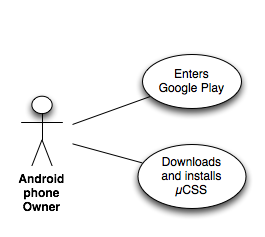
\includegraphics[scale=0.7]{images/UseCase1}
\caption[Yse case 1]{The user opens Google Play and finds and installs the $\mu$C Software Store application}
\end{figure}

The first use case describes how an Android-owner can browse Google Play to install the $\mu$C Software Store (abbr. $\mu$CSS).

    \begin{table}[H]
        \caption{Use case 1}
        \begin{tabularx}\linewidth{ |m{0.3 \textwidth} |X|   }
            \hline
                ID           & 1 \\
            \hline
                Name             & Install $\mu$CSS \\
            \hline
                Goal             & Have $\mu$CSS installed on the Android device\\
            \hline
                Actors           & Android device owner\\
            \hline
                Prerequisite     & The actor have a Android device with Google Play\\
            \hline
                Main Flow        &  1. Opens Google Play \\
                                 &  2. Search for ``$\mu$C Software Store'' \\
                                 &  3. Installs the application \\
            \hline
                Alternative Flow & None\\
            \hline
                Parent UC        & None\\
            \hline
                Child UC         & All\\
            \hline
        \end{tabularx}
    \end{table}

\begin{figure}[H]
\centering
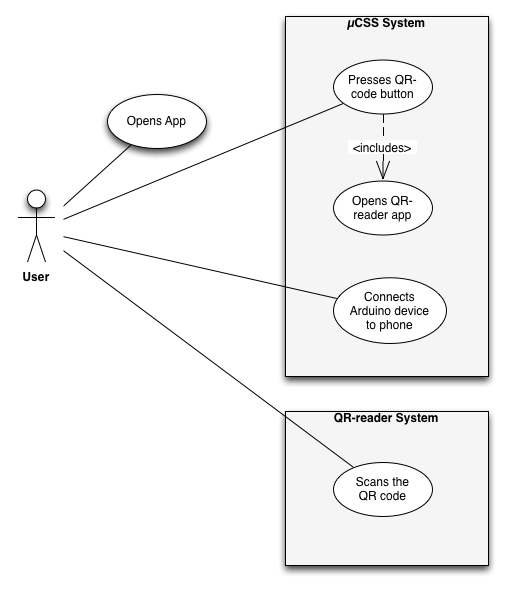
\includegraphics[scale=0.7]{images/UseCase2}
\caption[Use case 2]{The user connects to the Arduino with QR code}
\end{figure}

The second use case describes how the user can connect to an Arduino-device trough the $\mu$C Software Store, by using a previously downloaded QR Code reader on an Android. The $\mu$CSS automatically detects available QR Code readers on the Android device, and prompts the user to choose a QR Code reader to complete the action. $\mu$CSS automatically detects the QR Code read by the included action, and determines whether or not this is a valid code for an Arduino device, and attempts to pair the Android with the Arduino. If there's no QR Code reader application installed on the Android, $\mu$CSS prompts the user to install one.

\begin{table}[H]
    \caption{Use case 2}
    \begin{tabularx}\linewidth{ |m{0.3 \textwidth} |X| }
        \hline
            ID               & 2 \\
        \hline
            Name             & Pair Arduino device and Android device with QR Code\\
        \hline
            Goal             & Connect the Arduino device to the Android application with the use of QR Code\\
        \hline
            Actors           & Arduino device owner\\
        \hline
            Prerequisite     & Installed $\mu$CSS \\
                             & Installed predefined QR-reader\\
        \hline
            End requirement  & The Arduino device is connected to the phone via Bluetooth \\
        \hline
            Main flow        &  1. User opens $\mu$CSS \\
                             &  2. User presses the button indicating that he wants to pair with the Arduino device using QR Code \\
                             &  3. The system opens the QR reader application \\
                             &  4. The QR reader application reads the QR Code and returns the information it contains\\
                             &  5. The system pairs with the Arduino device \\
        \hline
            Alternative flow &  3.a. The user does not have the right QR Code reader installed \\
                             &  3.b. The system prompts the user if he wants to install the QR Code reader \\
                             &  3.c. If no: stop \\
                             &  4.a. The QR reader is unable to read the QR Code \\
                             &  4.b. Try again or stop\\
        \hline
            Parent UC        & 1\\
        \hline
            Child UC         & 7\\
        \hline
    \end{tabularx}
\end{table}

\begin{figure}[H]
\centering
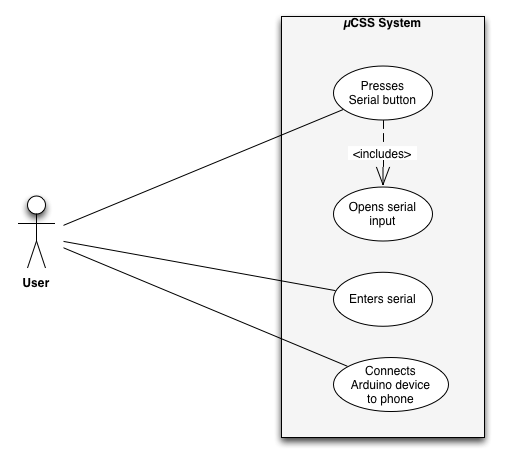
\includegraphics[scale=0.7]{images/UseCase3}
\caption[Use case 3]{The user connects to the Arduino with Serial input}
\end{figure}

The third use case describes how the user can connect to an Arduino-device trough the $\mu$C Software Store, by inputting the MAC address of the device. $\mu$CSS determines whether or not this is a valid MAC address, and attempts to pair the Android with the Arduino. If the MAC address is invalid, $\mu$CSS prompts the user to retry input.

\begin{table}[H]
    \caption{Use case 3}
    \begin{tabularx}\linewidth{ |m{0.3 \textwidth} |X| }
        \hline
            ID               & 3 \\
        \hline
            Name             & Pair Arduino device with Android device using serial \\
        \hline
            Goal             & Connect the Arduino device to the Android application with the use of QR Code \\
        \hline
            Actors           & Arduino device owner \\
        \hline
            Prerequisite     & Installed $\mu$CSS \\
                             & Installed predefined QR-reader \\
        \hline
            End requirement  & The Arduino device is connected to the phone via Bluetooth \\
        \hline
            Main flow        &  1. User opens $\mu$CSS \\
                             &  2. User presses the button indicating that he
                                    wants to pair with the Arduino device using a serial code \\
                             &  3. System opens dialog box for input\\
                             &  4. The user types the serial \\
                             &  5. The system pairs with the Arduino device \\
        \hline
            Alternative flow &  4.a. The user misspells the serial \\
                             &  4.b. The system displays an error, and prompts again \\
        \hline
            Parent UC        & 1 \\
        \hline
            Child UC         & 7 \\
        \hline
    \end{tabularx}
\end{table}

\begin{figure}[H]
\centering
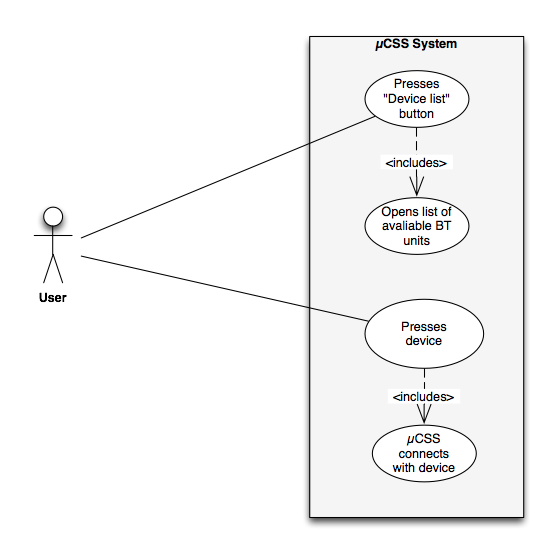
\includegraphics[scale=0.7]{images/UseCase7}
\caption[Use case 4]{User uses the bluetooth to scan for available connections.}
\end{figure}

The fourth use case describes how the user can choose an Arduino device from a list of available Bluetooth devices, and pair devices, from the menu in $\mu$CSS. 

\begin{table}[H]
    \caption{Use case 4}
    \begin{tabularx}\linewidth{ |m{0.3 \textwidth} |X| }
        \hline
            ID               & 4 \\
        \hline
            Name             & Pair Arduino device with Android device using device list \\
        \hline
            Goal             & Connect the Arduino device to the Android application with the use of device list \\
        \hline
            Actors           & Arduino device owner \\
        \hline
            Prerequisite     & Installed $\mu$CSS \\
        \hline
            End requirement  & The Arduino device is connected to the phone via Bluetooth \\
        \hline
            Main flow        &  1. User opens $\mu$CSS \\
                             &  2. User presses the device list button \\
                             &  3. System opens the list of available Bluetooth devices\\
                             &  4. The user presses the device to connect to \\
                             &  5. The system pairs with the Arduino device \\
        \hline
            Alternative flow &  None \\
        \hline
            Parent UC        & 1 \\
        \hline
            Child UC         & 7 \\
        \hline
    \end{tabularx}
\end{table}

\begin{figure}[H]
\centering
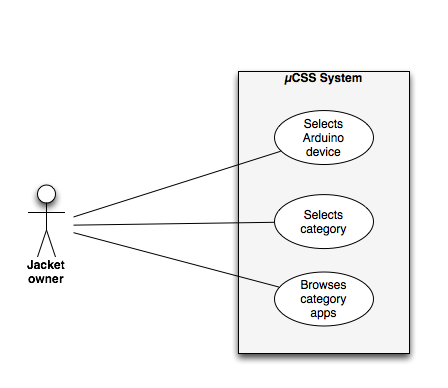
\includegraphics[scale=0.7]{images/UseCase4}
\caption[Use case 5]{The user selects a category and browses the applications}
\end{figure}

The fifth use case describes how the user can browse apps in the $\mu$CSS, and filter them on categories. Browsing of apps can be done both with or without pairing of an Arduino device.

        \begin{table}[H]
                \caption{Use case 5}
        \begin{tabularx}\linewidth{ |m{0.3 \textwidth} |X| }
            \hline
                ID               & 5 \\
            \hline
                Name             & Browse apps \\
            \hline
                Actors           & Arduino device owner \\
            \hline
                Prerequisite     & Installed $\mu$CSS \\
            \hline
                End Requirement  & None \\
            \hline
                Main Flow        &  1. The user opens $\mu$CSS \\
                                 &  2. The user selects the an Arduino device \\
                                 &  3. The user selects category (One category is named ``all'') \\
                                 &  4. The user browses apps \\
            \hline
             Alternative Flow    & 2.a. The user does not select Arduino device, but browses anyway \\
           \hline
            Parent UC        & 1 \\
        \hline
            Child UC         & 7 \\
        \hline
        \end{tabularx}
    \end{table}



\begin{figure}[H]
\centering
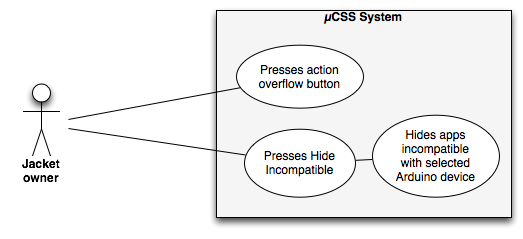
\includegraphics[scale=0.7]{images/UseCase5}
\caption[Use case 6]{The user can open the action overflow bar and hide/show incompatible applications}
\end{figure}

The sixth use case describes how the user can choose to filter apps in $\mu$CSS based on their compatibility with the paired Arduino device.

\begin{table}[H]
                \caption{Use case 6}
        \begin{tabularx}\linewidth{ |m{0.3 \textwidth} |X| }
            \hline
                ID               & 6 \\
            \hline
                Name             & Hide incompatible apps \\
            \hline
                Actors           & Arduino device owner \\
            \hline
                Prerequisite       & Installed $\mu$CSS \\
            \hline
                End Requirement  & None \\
            \hline
                Main Flow        &  1. The user presses action overflow button \\
                                 &  2. The user selects hide incompatible applications \\
                                 &  3. The application hides all incompatible applications from the user \\
                                 &  4. The user browses compatible apps \\
            \hline
             Alternative Flow    & none \\
           \hline
            Parent UC        & 1 \\
        \hline
            Child UC         & None \\
        \hline
        \end{tabularx}
    \end{table}

\begin{figure}[H]
\centering
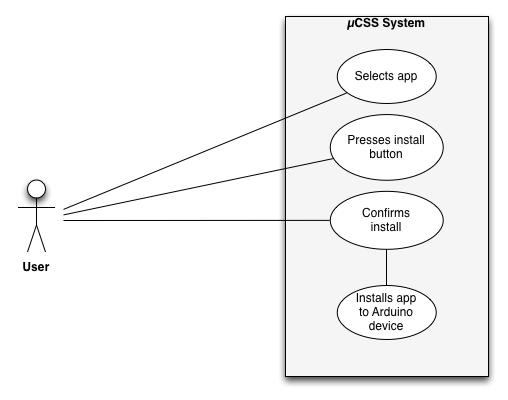
\includegraphics[scale=0.7]{images/UseCase6}
\caption[Use case 7]{The user selects an application, presses the install button and confirms it.}
\end{figure}

The seventh use case describes the user sequence to choose and install an application from the $\mu$CSS to the paired Arduino device.

\begin{table}[H]
    \caption{Use case 7}
    \begin{tabularx}\linewidth{ |m{0.3 \textwidth} |X| }
        \hline
            ID               & 7 \\
        \hline
            Name             & Install application on Arduino device \\
        \hline
            Goal             & Connect the Arduino device to the Android application with the use of QR Code \\
        \hline
            Actors           & Arduino device owner \\
        \hline
            Prerequisite     &  Installed $\mu$CSS \\
                             &  Arduino device connected to $\mu$CSS \\
        \hline
            End requirement  & The application is installed on the Arduino device \\
        \hline
            Main flow        &  The user selects the desired application \\
                             &  The user presses the ``install'' button \\
                             &  The user confirms the installation \\
                             &  The application is installed at the Arduino device \\
        \hline
            Alternative flow & none \\
        \hline
            Parent UC        & 1, 2, 3, 4, 5, 6 \\
        \hline
            Child UC         & None \\
        \hline
    \end{tabularx}
\end{table}

\begin{figure}[H]
\centering
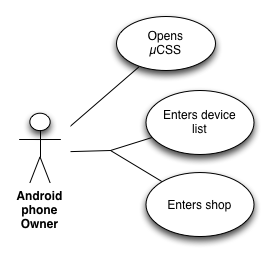
\includegraphics[scale=0.7]{images/UseCase_welcome_screen}
\caption[Use case 8]{When the user starts the application this screen will be shown where the user can choose to select device list or browse the shop.}
\end{figure}

The eighth use case is the welcome screen which shows every time $\mu$CSS is opened. 

\begin{table}[H]
    \caption{Use case 8}
    \begin{tabularx}\linewidth{ |m{0.3 \textwidth} |X| }
        \hline
            ID               & 8 \\
        \hline
            Name             & Welcome screen \\
        \hline
            Goal             & Open the application \\
        \hline
            Actors           & Android application owner \\
        \hline
            Prerequisite     &  Installed $\mu$CSS \\
        \hline
            End requirement  & The application is opened \\
        \hline
            Main flow        &  The user selects the $\mu$CSS application \\
                             & $\mu$CSS is opened and the welcome screen is displayed\\
        \hline
            Alternative flow & none \\
        \hline
            Parent UC        & 1 \\
        \hline
            Child UC         & 2, 3, 4, 5, 6, 7 \\
        \hline
    \end{tabularx}
\end{table}
